\documentclass{beamer}

\usepackage{float}
\usepackage{listings}
\usepackage{hyperref}
\usepackage{graphicx}
\usepackage{tikz,times}
\usepackage{amsmath}
\usepackage{xspace}
\usepackage{array}

\mode<presentation>
{
  \usetheme{Warsaw} 
  \setbeamercovered{transparent}
}

\AtBeginSection{
\begin{frame}<beamer>{Outline}
  \tableofcontents[currentsection,currentsubsection]
\end{frame}
}


\title[]{Deep Learning lab}
\subtitle{}

\author[Uni-Freiburg]{Mostafa Mohamed, Omar Kassem}
\date{\today}
\institute{Alberts-Ludwig Universt\"at Freiburg}

%\usecolortheme{Copenhagen}


%\usetheme{EastLansing}
\usepackage{natbib}
\bibliographystyle{apalike}
% make bibliography entries smaller
\renewcommand\bibfont{\scriptsize}
% If you have more than one page of references, you want to tell beamer
% to put the continuation section label from the second slide onwards
\setbeamertemplate{frametitle continuation}[from second]
% Now get rid of all the colours
\setbeamercolor*{bibliography entry title}{fg=black}
\setbeamercolor*{bibliography entry author}{fg=black}
\setbeamercolor*{bibliography entry location}{fg=black}
\setbeamercolor*{bibliography entry note}{fg=black}
% and kill the abominable icon
\setbeamertemplate{bibliography item}{}

\begin{document}

\begin{frame}
\titlepage
\end{frame}

\begin{frame}{Outline}
  \setcounter{tocdepth}{1}
  \tableofcontents
\end{frame}

\section{Introduction}
\begin{frame}{Problem Statement}
\begin{enumerate}
\item Visual planning imitating A*
\item Changing target
\end{enumerate}
\begin{figure}
        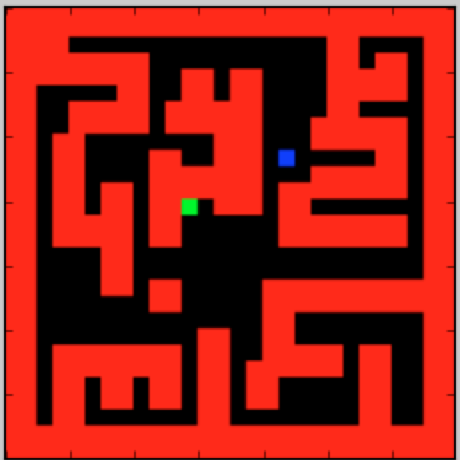
\includegraphics[width=0.30\linewidth]{problem.png}
    \label{fig1}
\end{figure}
\end{frame}

\begin{frame}{Old results}
\begin{itemize}
    \item The A* star was our baseline for training, it always solves the problem.
    \item The accuracy of our agent without changing the target was 100\%.
    \item The accuracy of our agent with changing target was on average 31\%.
\end{itemize}
\end{frame}

\section{Storing target}
\begin{frame}{Adding target to state}
In addition to the history of the last 4 states, we save an additional state of the local view of the target position.
Average accuracy with saving target: 70\%
Average accuracy : 31\%
\end{frame}

\section{Coloring}
\begin{frame}{Simple coloring}
Dividing the wall into "districts" with distinct colors.\\
Average accuracy with colouring: 81\%

Average accuracy : 31\%
\begin{figure}
        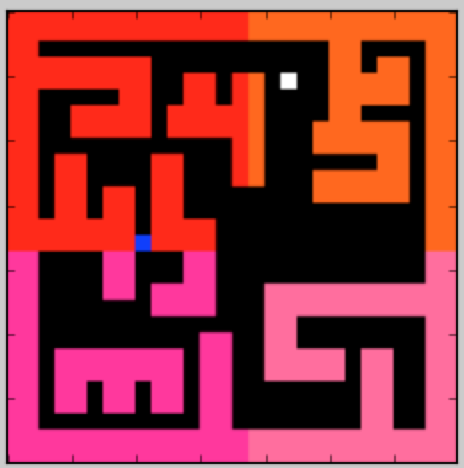
\includegraphics[width=0.35\linewidth]{simple.png}
        \caption{Simple colouring}
    \label{fig1}
\end{figure}
\end{frame}

\begin{frame}{Gradient coloring}
Coloring the walls with a gradient across the whole map. \\
Average accuracy with colouring: 66\%

Average accuracy : 31\%
\begin{figure}
        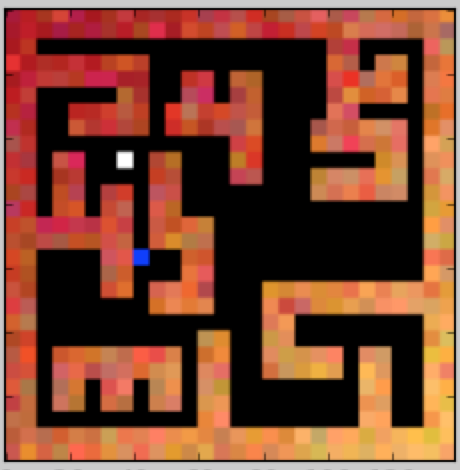
\includegraphics[width=0.35\linewidth]{gradient.png}
        \caption{Gradient colouring}
    \label{fig2}
\end{figure}
\end{frame}

\section{Gridding}
\begin{frame}{Distance accuracy}
    \begin{itemize}
        \item Instead of giving a score 0 for not reaching the target, we use the distance accuracy function: $$\frac{1}{1 + {\lfloor d/g \rfloor}^2}$$ where $d$ is the distance from the target and $g$ is a constant.
        \item The idea is to give partial credit if the agent got close to the target even if it didn't reach it. 
    \end{itemize}
\end{frame}

\begin{frame}{Gridding}
\begin{itemize}
    \item We tried to divide the map into grids of size $g$ while sampling target locations (only during training).
    \item The reason is to ensure that the density of distribution across the map is the same.
    \item However it turns out that gridding didn't affect the results that much.
\end{itemize}
\end{frame}

\section{Final results}
\begin{frame}
We ran 8 experiments; for each we train 7 times and test 10 for each of them, and these are the average results.
\begin{center}
    \begin{tabular}{| l | l | l | l | l |}
    \hline
    Target & Gridding & Color & Accuracy & Distance Accuracy \\ \hline
    No & No & No & 31\% & - \\ \hline
    Yes & No & No & 70\% & - \\ \hline
    Yes & No & Simple & 80\% & - \\ \hline
    Yes & No & Gradient & 66\% & - \\ \hline
    Yes & Yes & Simple & 79\% & 81\% \\ \hline
    Yes & Big& Simple & 77\% & 82\% \\ \hline
    Yes & Yes & No & 70\% & 72\% \\ \hline
    Yes & Big & Gradient & 64\% & 71\% \\ \hline
    \end{tabular}
\end{center}
\end{frame}

\iffalse
\begin{frame}{Recall}
\begin{figure}
        \includegraphics{train_test.png}
        \caption{Train and Test recall}
    \label{fig1}
\end{figure}
\end{frame}

\begin{frame}{Top 200 Recall}
\begin{figure}
        \includegraphics{recall200.png}
        \caption{Top 200 Recall}
    \label{fig1}
\end{figure}
\end{frame}

\begin{frame}{MRR, nDCG @ 5}
\begin{figure}
        \includegraphics{mrrndcg5.png}
        \caption{MRR, nDCG @ 5}
    \label{fig1}
\end{figure}
\end{frame}

\begin{frame}{MRR, nDCG @ 10}
\begin{figure}
        \includegraphics{mrrndcg10.png}
        \caption{MRR, nDCG @ 10}
    \label{fig1}
\end{figure}
\end{frame}
\fi
\begin{frame}
We also tried a bigger map
\begin{figure}
        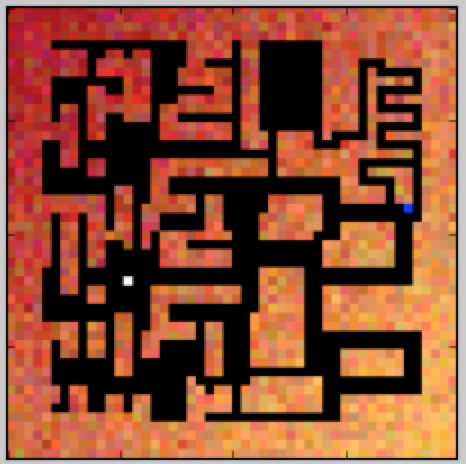
\includegraphics[width=0.45\linewidth]{bigmap.png}
    \label{fig2}
\end{figure}
\end{frame}


\end{document}
